% This template is indended for writting the the project report in ``Machine Learning``
%
% It is based on the MikTex ``article`` template, modified with content from the DIT ``Studienarbeit`` template, originally created by Prof. Dr. Andreas Fischer.
%
% Markus Mayer, 2022-03-23

\documentclass[11pt]{article} % use larger type; default would be 10pt
\usepackage[utf8]{inputenc} % set input encoding (not needed with XeLaTeX)

%%% Examples of Article customizations
% These packages are optional, depending whether you want the features they provide.
% See the LaTeX Companion or other references for full information.

%%% PAGE DIMENSIONS
\usepackage{geometry} % to change the page dimensions
\geometry{a4paper} % or letterpaper (US) or a5paper or....
% \geometry{margin=2in} % for example, change the margins to 2 inches all round
% \geometry{landscape} % set up the page for landscape
%   read geometry.pdf for detailed page layout information

\usepackage{graphicx} % support the \includegraphics command and options
\DeclareGraphicsExtensions{.pdf,.png,.jpg}

% \usepackage[parfill]{parskip} % Activate to begin paragraphs with an empty line rather than an indent

%%% PACKAGES
\usepackage{algorithmic} % For pseudo code
\usepackage{amsmath}
\usepackage{booktabs} % for much better looking tables
\usepackage{array} % for better arrays (eg matrices) in maths
\usepackage{paralist} % very flexible & customisable lists (eg. enumerate/itemize, etc.)
\usepackage{verbatim} % adds environment for commenting out blocks of text & for better verbatim
\usepackage{subfig} % make it possible to include more than one captioned figure/table in a single float
\usepackage{url}
\usepackage{hyperref}
\usepackage{float}
% These packages are all incorporated in the memoir class to one degree or another...

%%% HEADERS & FOOTERS
\usepackage{fancyhdr} % This should be set AFTER setting up the page geometry
\pagestyle{fancy} % options: empty , plain , fancy
\renewcommand{\headrulewidth}{0pt} % customise the layout...
\lhead{}\chead{}\rhead{}
\lfoot{}\cfoot{\thepage}\rfoot{}

%%% SECTION TITLE APPEARANCE
\usepackage{sectsty}
\allsectionsfont{\sffamily\mdseries\upshape} % (See the fntguide.pdf for font help)
% (This matches ConTeXt defaults)

%%% ToC (table of contents) APPEARANCE
\usepackage[nottoc,notlof,notlot]{tocbibind} % Put the bibliography in the ToC
\usepackage[titles,subfigure]{tocloft} % Alter the style of the Table of Contents
\renewcommand{\cftsecfont}{\rmfamily\mdseries\upshape}
\renewcommand{\cftsecpagefont}{\rmfamily\mdseries\upshape} % No bold!

%%% END Article customizations

%%% The "real" document content comes below...
\title{Project report on\\
song popularity classification \\
}
\author{Omar Chafik, Santiago Lema}
\date{\today}

\begin{document}
\maketitle

\section{Introduction}

Throughout history, music has held a profound place in human society, transcending cultural boundaries and serving as a fundamental means of expression and engagement. From ancient tribal rituals to modern-day streaming platforms, music has always captivated our hearts and souls. It has the unique ability to evoke emotions, connect people, and create shared experiences.

In today's digital age, the music industry has witnessed (and continues to witness) a deep transformation, where engagement and popularity on digital platforms play a crucial role in an artist's success. With millions of songs available on these platforms, understanding the factors that drive popularity and listeners' willingness to engage with a song is of great interest to artists, record labels, and other stakeholders in the music industry.

This project aims to delve into the realm of music popularity prediction, focusing on songs available on Spotify and YouTube, analyzing the relation between music features and users preferences. The goal will be pursued by developing  a classification model capable of predicting the popularity segment of a song, based on selected features. This entails constructing a comprehensive dataset containing various features and attributes of songs from the mentioned platforms. Leveraging such machine learning techniques, we will explore and compare multiple classification models to identify the most effective approach. Furthermore, we will fine-tune the selected models to extract the best possible results.

The motivation for this problem statement is to understand better  what makes a song successful on different platforms and to potentially use this information to inform marketing strategies for artists and record labels.

Also, this is an exciting opportunity to merge music, data science and industry insights to gain a better understanding of the factors which give life to this ancient form of art.

The ground set of data for this project was obtained from a pre-built dataset available in Kaggle called \textit{Spotify and Youtube}, authored by Salvatore Rastelli\cite{Rasetri}. The data was collected in February of 2023 so it is relatively recent to the production of this document. However, we are aware that new content was released in the meantime so we considered using more recent data for testing the model.

\section{Data}

Diving deeper into the dataset, it contains 20.718 songs with the following features:

\begin{table}[H]
	\centering
	\begin{tabular}{lcc}
		\toprule
		\textbf{Attribute} & \textbf{Unique values} & \textbf{Description}                             \\
		\midrule
		Artist             & 2079                   & Name of the artist                               \\
		Url\_spotify       & 2079                   & Spotify URL for the song                         \\
		Track              & 17841                  & Name of the track                                \\
		Album              & 11937                  & Name of the album                                \\
		Album\_type        & 3                      & Type of the album                                \\
		Uri                & 18862                  & URI of the song                                  \\
		Danceability       & 898                    & Measure of the song's danceability               \\
		Energy             & 1268                   & Measure of the song's energy                     \\
		Key                & 12                     & Key of the song                                  \\
		Loudness           & 9417                   & Loudness level of the song                       \\
		Speechiness        & 1303                   & Measure of the song's speechiness                \\
		Acousticness       & 3138                   & Measure of the song's acousticness               \\
		Instrumentalness   & 4012                   & Measure of the song's instrumentalness           \\
		Liveness           & 1536                   & Measure of the song's liveness                   \\
		Valence            & 1293                   & Measure of the song's valence                    \\
		Tempo              & 15024                  & Tempo of the song                                \\
		Duration\_ms       & 14690                  & Duration of the song in milliseconds             \\
		Url\_youtube       & 18154                  & YouTube URL for the song                         \\
		Title              & 18146                  & Title of the YouTube video                       \\
		Channel            & 6714                   & YouTube channel of the uploader                  \\
		Views              & 19245                  & Number of views on YouTube                       \\
		Likes              & 17939                  & Number of likes on YouTube                       \\
		Comments           & 10485                  & Number of comments on YouTube                    \\
		Description        & 17395                  & Description of the YouTube video                 \\
		Licensed           & 2                      & Indicates if the song is licensed                \\
		official\_video    & 2                      & Indicates if it's an official video              \\
		Stream             & 18461                  & Indicates if the song is available for streaming \\
		\bottomrule
	\end{tabular}
	\caption{Attributes of the dataset}
	\label{tab:attributes}
\end{table}

The features of highest interest for the purpose of this project are the numerical ones, but we will also use some of the categorical.
Some of these features refer to specific terminology used in the music industry to describe characteristics of a song.
The following list, took from Spotify API's Documentation \cite{spotifyApi} provides a brief explanation of these terms:

\begin{itemize}
	\item \textit{Danceability}: describes how suitable a track is for dancing based on a combination of musical elements including tempo, rhythm stability, beat strength, and overall regularity. A value of 0.0 is least danceable and 1.0 is most danceable.
	\item \textit{Energy}: is a measure from 0.0 to 1.0 and represents a perceptual measure of intensity and activity. Typically, energetic tracks feel fast, loud, and noisy. For example, death metal has high energy, while a Bach prelude scores low on the scale. Perceptual features contributing to this attribute include dynamic range, perceived loudness, timbre, onset rate, and general entropy.
	\item \textit{Key}: the key the track is in. Integers map to pitches using standard Pitch Class notation. E.g. 0 = C, 1 = C\# , 2 = D, and so on. If no key was detected, the value is -1.
	\item \textit{Loudness}: the overall loudness of a track in decibels (dB). Loudness values are averaged across the entire track and are useful for comparing relative loudness of tracks. Loudness is the quality of a sound that is the primary psychological correlate of physical strength (amplitude). Values typically range between -60 and 0 db.
	\item \textit{Speechiness}: detects the presence of spoken words in a track. The more exclusively speech-like the recording (e.g. talk show, audio book, poetry), the closer to 1.0 the attribute value. Values above 0.66 describe tracks that are probably made entirely of spoken words. Values between 0.33 and 0.66 describe tracks that may contain both music and speech, either in sections or layered, including such cases as rap music. Values below 0.33 most likely represent music and other non-speech-like tracks.
	\item \textit{Acousticness}: a confidence measure from 0.0 to 1.0 of whether the track is acoustic. 1.0 represents high confidence the track is acoustic.
	\item \textit{Instrumentalness}: predicts whether a track contains no vocals. "Ooh" and "aah" sounds are treated as instrumental in this context. Rap or spoken word tracks are clearly "vocal". The closer the instrumentalness value is to 1.0, the greater likelihood the track contains no vocal content. Values above 0.5 are intended to represent instrumental tracks, but confidence is higher as the value approaches 1.0.
	\item \textit{Liveness}: detects the presence of an audience in the recording. Higher liveness values represent an increased probability that the track was performed live. A value above 0.8 provides strong likelihood that the track is live.
	\item \textit{Valence}: a measure from 0.0 to 1.0 describing the musical positiveness conveyed by a track. Tracks with high valence sound more positive (e.g. happy, cheerful, euphoric), while tracks with low valence sound more negative (e.g. sad, depressed, angry).
	\item \textit{Tempo}: the overall estimated tempo of a track in beats per minute (BPM). In musical terminology, tempo is the speed or pace of a given piece and derives directly from the average beat duration.
\end{itemize}

The histograms observed in Figure 1 show the distribution of the main numerical attributes in the dataset will help to get a better understanding of the initial state of the data.
\begin{figure}[ht]
	\centering
	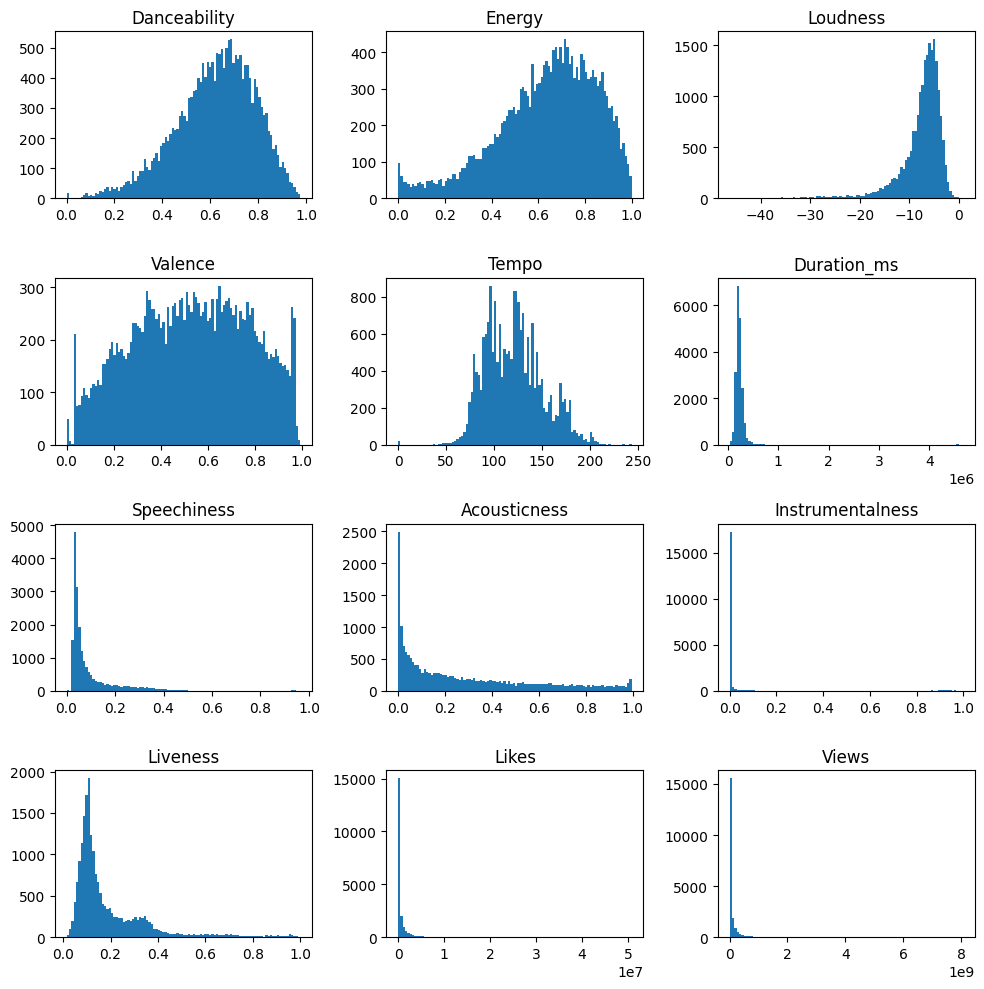
\includegraphics[width=.8\linewidth]{numeric_variables_histograms.png}
	\caption{Histograms of main numerical attributes}\label{fig:numeric_variables_histograms}
\end{figure}

As it can be seen, there is no specific target variable in the dataset. Earlier, when the goal was stated (predicting the popularity of a song), the actual definition of popularity was not mentioned. As a matter of fact, it is not easy to define the popularity of a song in a particular digital platform.
Because of this subjectivity of the concept which is trying to be predicted, we will mention a series of definitions that were considered to eventually justify a more objective definition of the target variable \textit{popularity}.

In the English language, according to the Cambridge Dictionary \cite{CambridgeDictionary}, popularity is "the fact that something or someone is liked, enjoyed, or supported by many people".

In the Collins Dictionary \cite{CollinsDisctionary}, the definition that can be found is that "something that is popular is enjoyed or liked by a lot of people".

In a sociologic context, paraphrasing Wikipedia \cite{WikipediaPopularity}, popularity, derived from the Latin term \textit{popularis} meaning "common," has evolved to signify the "fact or condition of being well liked by the people". Although popularity is often attributed to individuals, it is fundamentally a social phenomenon that can only be comprehended within the context of groups. Popularity is a collective perception, and individuals gauge the consensus of a group's sentiments when assessing popularity of an individual or object. The degree of advocacy and positive opinions expressed by a group directly influences the attention and level of popularity something or someone attains.

However, popularity extends beyond individuals and can be attributed to various objects such as songs, movies, websites, activities, soaps, foods, and more. These objects collectively form popular culture, representing the prevailing preferences within society. Essentially, anything, whether human or non-human, has the potential to be regarded as popular.

Given these definitions, there are more basis to argue that popularity can exist as an attribute of a song if it helps measuring the degree of advocacy and positive opinions expressed by a group of people. In this case, the group of people will be the users of the digital platforms Spotify and YouTube, and the appreciation will be measured by the number of likes and views.
In order to detail this process, first we can analyze these two variables further as they became now more relevant.

In the previous histograms it could be noticed a peculiar distribution for the likes and views. They can be better appreciated in the following rug plots.

\begin{figure}[ht]
	\centering
	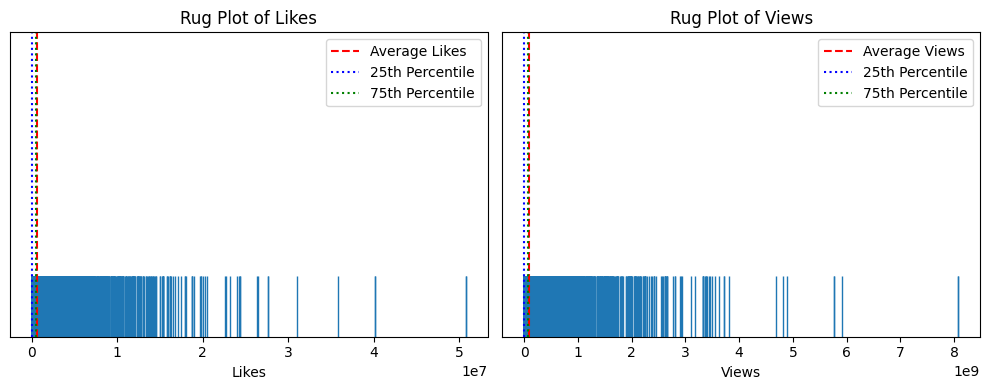
\includegraphics[width=.8\linewidth]{rug_plots_views_likes.png}
	\caption{Distribution of likes and views}\label{fig:rug_plots_views_likes}
\end{figure}

It is undoubtedly a very skewed distribution, with a very high concentration of values in the lower part of the range. This is a very common behavior in social media platforms, where the majority of the content is not popular and only a few pieces of content become viral.

This is also known as the \textit{long tail} phenomenon, which is a characteristic of power law distributions \cite{LongTail}.

If we take a look at the statistics of these two variables, we can see that the mean is much higher than the median, which is a clear indicator of the skewness of the distribution, and also the last quartile is distributed in a much broader range of values.

\begin{table}[H]
	\centering
	\begin{tabular}{lcc}
		\toprule
		Attribute & Likes             & Views             \\
		\midrule
		Count     & 20177.0           & 20177.0           \\
		Mean      & $6.633\times10^5$ & $9.418\times10^7$ \\
		Std       & $1.789\times10^6$ & $2.750\times10^8$ \\
		Min       & 0.0               & 0.0               \\
		25\%      & 21581.0           & 1835998.0         \\
		50\%      & 124481.0          & 14542507.0        \\
		75\%      & 522148.0          & 70572997.0        \\
		Max       & $5.078\times10^7$ & $8.079\times10^9$ \\
		\bottomrule
	\end{tabular}
	\caption{Basic Statistics for Likes and Views}
	\label{tab:stats}
\end{table}

To assess the popularity of songs given these attributes, a third attribute called "Popularity score" was developed. This score is calculated by weighting the likes and views. Comments were excluded based on the understanding that, according to established definitions of popularity, only positive comments would contribute to the popularity score. Conducting sentiment analysis on the comments was beyond the scope of this project and not feasible due to data limitations.

The weights initially assigned to likes and views were 0.7 and 0.3, respectively. This choice of weights was subjective and based on the interpretations of the definitions mentioned earlier. According to these definitions, popularity is primarily associated with liking or enjoying something, rather than the sheer quantity of views or spread of the content.

It is important to note that these weightings were determined based on a subjective decision and may vary depending on the context or specific goals of future analyses.

This score served as the basis for creating the target variable "popularity." The target variable was transformed into a categorical value that defines distinct zones or neighborhoods of popularity. Initially, the popularity variable was categorized into four values: "Low," "Moderate," "High," and "Very high." These categories corresponded to specific thresholds based on the distribution of the popularity score. The thresholds were set as follows: the lowest 30\% of popularity scores fell into the "Low" category, popularity scores between 30% and 70% were classified as "Moderate," scores between 70% and 90% fell into the "High" category, and the top 10% of popularity scores were classified as "Very high."

This approach allowed for the creation of discrete popularity levels, enabling a more nuanced analysis of the songs' popularity within distinct tiers. It should be noted that these threshold values and the number of categories were determined based on the specific distribution of the popularity score in the dataset. Alternative categorizations could be explored depending on the specific requirements of future analyses or applications.

\begin{table}[H]
	\centering
	\begin{tabular}{lc}
		\toprule
		\textbf{Popularity category} & \textbf{Values count} \\
		\midrule
		Low                          & 6053                  \\
		Moderate                     & 8071                  \\
		High                         & 4035                  \\
		Very high                    & 2018                  \\
		\bottomrule
	\end{tabular}
	\caption{Popularity count by category}
	\label{tab:stats}
\end{table}

To ensure a focused and effective data preprocessing phase, certain attributes were removed from the dataset. Initially, categorical attributes that were not planned to be used in the classification model were eliminated. These included the artist name, URLs, URIs, track numbers, and album names. As these attributes did not contribute directly to the classification task, their removal helped streamline the dataset and reduce unnecessary complexity.

Furthermore, the attributes related to likes, comments, and views were also excluded from the dataset. These attributes were expected to exhibit high correlation with the popularity score, as they are potential indicators or direct factors contributing to the determination of popularity. By removing these attributes, we aimed to avoid issues of multicollinearity and prevent the classification model from relying too heavily on features that directly represent the target variable.

\begin{figure}[H]
	\centering
	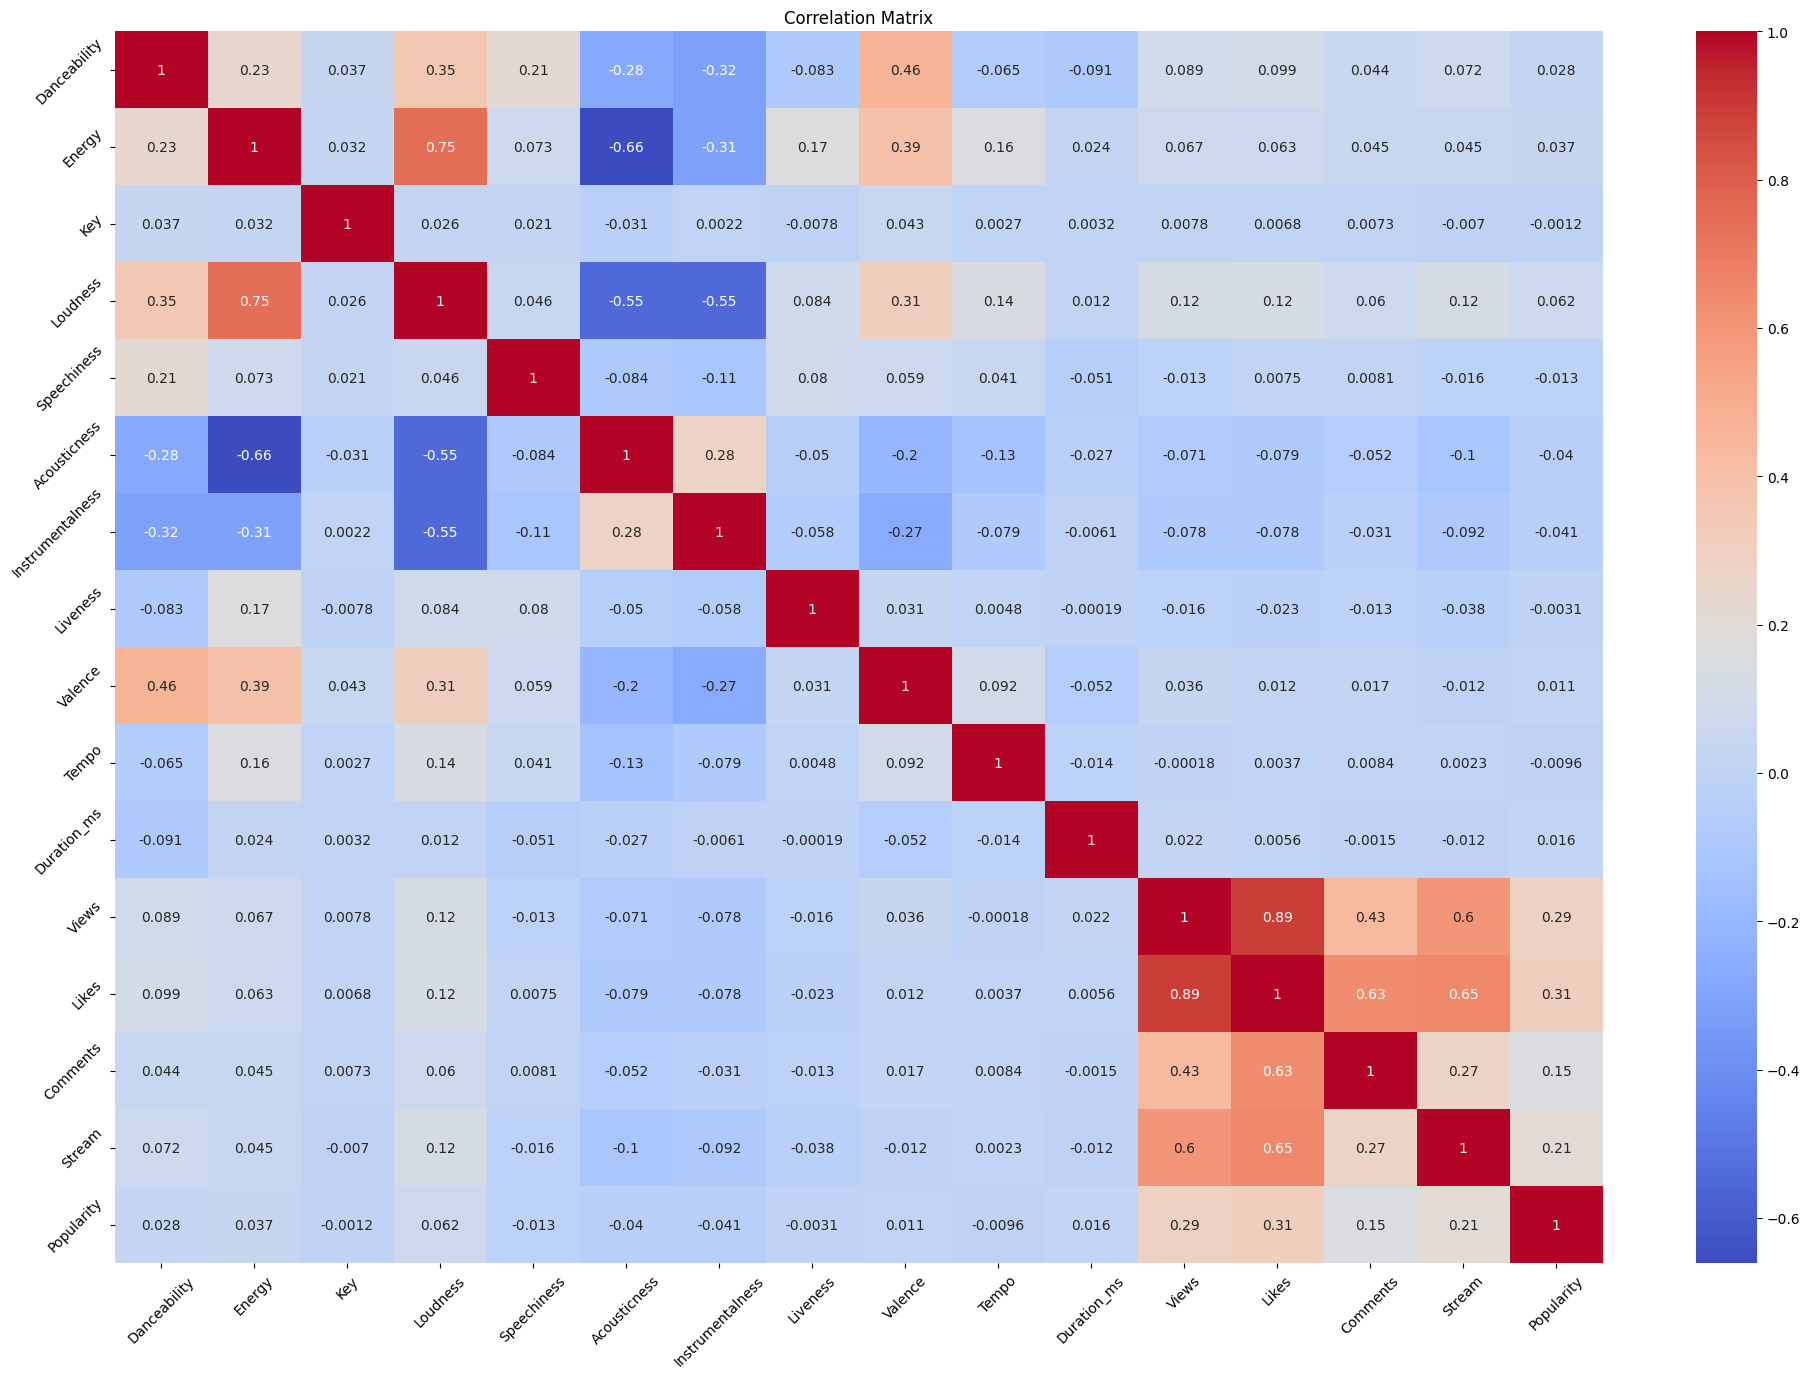
\includegraphics[width=.8\linewidth]{correlation_matrix.png}
	\caption{Correlation matrix}\label{fig:correlation_matrix}
\end{figure}

This preprocessing step allowed us to create a more refined dataset, focusing on the most relevant attributes for the classification model. By eliminating unnecessary categorical attributes and features highly correlated with the target variable, we aimed to enhance the model's performance and interpretability.


\section{Method}

In tackling the classification problem, we carefully selected several models to implement and subsequently compare their performance. The chosen models for this task include Support Vector Machine (SVM), Random Forest, and K-Nearest Neighbors (KNN).

Each of these models offers distinct advantages that make them suitable for our problem:

\begin{itemize}
	\item Support Vector Machine (SVM): SVM is a powerful and versatile classification algorithm known for its ability to handle complex datasets and find optimal decision boundaries. It is particularly effective when dealing with high-dimensional data and can handle both linear and non-linear classification problems. SVM aims to maximize the margin between different classes, thereby promoting robustness and generalizability in the classification process.
	\item Random Forest: Random Forest is an ensemble learning method that combines multiple decision trees to make predictions. It excels in handling large and diverse datasets while avoiding overfitting. By using bootstrap sampling and feature randomization, Random Forest mitigates the risk of variance and bias, providing robust and accurate predictions. It is particularly useful when dealing with complex relationships and feature interactions.
	\item K-Nearest Neighbors (KNN): KNN is a non-parametric algorithm that classifies data points based on their proximity to other labeled instances. It is an intuitive and easy-to-understand method that requires no training phase. KNN works well with datasets where instances with similar features tend to have the same label. It is also effective when the decision boundaries are irregular or nonlinear. KNN allows for flexibility in defining the value of K, the number of nearest neighbors considered during classification.
\end{itemize}

After running all these, we will compare the results and choose the best model to fine-tune it and get the best possible results. However, before running the models, additional preprocessing steps were performed. For categorical variables, encoding techniques were applied. The target variable was encoded using label encoding, while the remaining categorical variables were encoded using one-hot encoding.

Label encoding was chosen for the target variable as it is a categorical variable with ordinal levels. Label encoding assigns a unique numerical label to each category, thereby preserving the ordinal relationship between the categories. This encoding allows the classification models to interpret the target variable correctly during training and prediction.

On the other hand, one-hot encoding was used for the remaining categorical variables. One-hot encoding creates binary dummy variables for each category, representing the presence or absence of that category in a given observation. This encoding scheme is suitable for non-ordinal categorical variables as it prevents the models from assigning any arbitrary ordinal relationship among the categories.

Regarding the numerical values, a normalization technique was applied specifically for the KNN model. Normalization ensures that all numerical features have a similar scale, which is crucial for distance-based algorithms like KNN. By scaling the numerical values to a standard range (e.g., between 0 and 1), the KNN algorithm can give equal importance to each feature during classification, preventing features with larger scales from dominating the distance calculations.

Overall, by encoding the categorical variables and applying normalization to the numerical values, the data was prepared appropriately for the selected models. These preprocessing steps aim to enhance the models' performance and ensure they can effectively learn from the data, leading to more accurate predictions of song popularity.

Almost ready to go through the models, the dataset was split into an 80/20 ratio, with 80\% of the data used for training the models and 20\% held out for testing purposes. This serves to evaluate the model's performance on unseen data. The selected ratio 80/20 is meant to strike a balance between having sufficient data for training the models and having a reasonable amount of data for evaluation. With 80\% of the data allocated for training, the models can learn patterns and relationships from a substantial portion of the dataset, allowing them to capture the underlying trends in the data.

The remaining 20\% of the data, reserved for testing, serves as an independent sample to evaluate the models' performance. By assessing the models on unseen data, we can measure their ability to generalize and make accurate predictions on new instances. This helps us estimate how well the models will perform when applied to real-world scenarios or new data points.

\section{Results and conclusion}

The KNN model was evaluated using various performance metrics provided by the Python library \textit{Sklearn}. The results are presented in the following table:

\begin{table}[H]
	\centering
	\begin{tabular}{lcccc}
		\toprule
		\textbf{Popularity Level} & \textbf{Precision} & \textbf{Recall} & \textbf{F1-Score} & \textbf{Support} \\
		\midrule
		High Popularity           & 0.35               & 0.08            & 0.13              & 796              \\
		Low Popularity            & 0.57               & 0.51            & 0.53              & 1086             \\
		Moderate Popularity       & 0.44               & 0.75            & 0.56              & 1551             \\
		Very High Popularity      & 0.09               & 0.00            & 0.01              & 401              \\
		\hline
		Accuracy                  & -                  & -               & 0.47              & 3834             \\
		Macro Avg                 & 0.36               & 0.34            & 0.31              & 3834             \\
		Weighted Avg              & 0.42               & 0.47            & 0.40              & 3834             \\
		\bottomrule
	\end{tabular}
\end{table}

The precision metric measures the proportion of correctly predicted instances for each popularity level. Recall represents the percentage of instances correctly classified for a particular popularity level out of all instances belonging to that level. The F1-score combines both precision and recall, providing a balanced measure of the model's performance.

From the results, it can be observed that the KNN model achieved a relatively low precision for High Popularity and Very High Popularity levels, indicating that it struggled to accurately classify instances belonging to these categories. The recall for Very High Popularity was particularly worse, suggesting that the model failed drastically in identifying instances of the most popular songs.

On the other hand, the model performed relatively well in terms of precision and recall for Low Popularity and Moderate Popularity levels. These categories had higher F1-scores, indicating a better balance between precision and recall.

The overall accuracy of the KNN model was 0.47, indicating that it correctly classified approximately 47\% of the instances in the test set. The macro-average F1-score, which calculates the average F1-score across all popularity levels, was 0.31. The weighted average F1-score, which considers the proportion of instances in each popularity level, was 0.40.

These results reveal some limitations of the KNN model in predicting song popularity based on the given dataset, and particularly for the categories we are most interested in: instances belonging to the High Popularity and Very High Popularity songs.

\begin{figure}[H]
	\centering
	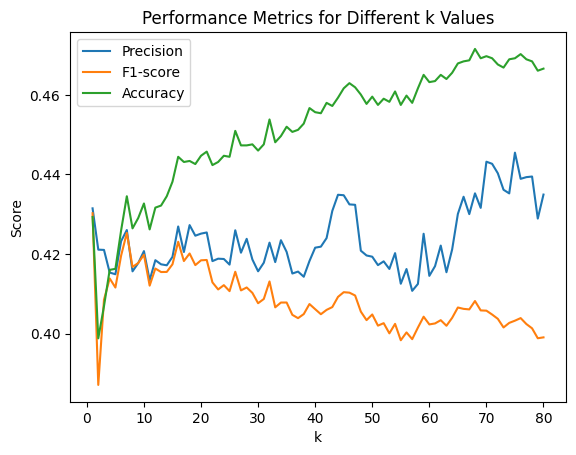
\includegraphics[width=.8\linewidth]{performance_different_k_values.png}
	\caption{KNN model performance across different k values}\label{fig:knn_k_selection}
\end{figure}

The parameter k, which represents the number of neighbors considered for classification in the KNN model, was selected by evaluating the model's performance across a range of values from 1 to 100. The k value that yielded the best performance was chosen as the optimal parameter for the final model. This process ensures that the model is tuned to the dataset and maximizes its predictive capabilities by considering an appropriate number of nearest neighbors for classification.

The SVG model, unfortunately, did not yield improved results compared to the KNN model. The classification report for the SVG model is as follows:

\newblock

\begin{table}[H]
	\centering
	\begin{tabular}{lcccc}
		\toprule
		\textbf{Popularity Level} & \textbf{Precision} & \textbf{Recall} & \textbf{F1-Score} & \textbf{Support} \\
		\midrule
		\hline
		High Popularity           & 0.86               & 0.01            & 0.01              & 796              \\
		Low Popularity            & 0.59               & 0.49            & 0.53              & 1086             \\
		Moderate Popularity       & 0.43               & 0.82            & 0.57              & 1551             \\
		Very High Popularity      & 1.00               & 0.00            & 0.00              & 401              \\
		\hline
		Accuracy                  & -                  & -               & 0.47              & 3834             \\
		Macro Avg                 & 0.72               & 0.33            & 0.28              & 3834             \\
		Weighted Avg              & 0.63               & 0.47            & 0.38              & 3834             \\
		\bottomrule
	\end{tabular}
\end{table}

The SVG model did not show better results compared to the KNN model. It struggled particularly with instances labeled as "Very High Popularity," as indicated by the precision of 1.0 and recall of 0.0 for this category. This means that while the model correctly predicted all instances it labeled as "Very High Popularity," it missed identifying any instances that actually belonged to this category. This could be due to the scarcity of instances labeled as "Very High Popularity" in the dataset, making it challenging for the model to learn and generalize patterns effectively.

For the other popularity levels, the SVG model performed reasonably well but still had room for improvement. It showed higher precision and recall for the "Moderate Popularity" category compared to the "High Popularity" and "Very High Popularity" categories. This indicates that the model was better at correctly classifying instances in the "Moderate Popularity" range. However, it still exhibited some misclassifications and struggled to achieve high precision and recall for the "High Popularity" category.

Overall, the accuracy of the SVG model was the same as the KNN model, indicating that both models correctly predicted approximately 47\% of instances in the test set.

\newblock

The random forest model yielded an accuracy of 0.532, indicating that it correctly predicted approximately 53.2\% of the instances in the test set and positioning as the best performer of the models.

\begin{table}[H]
	\centering
	\begin{tabular}{lcccc}
		\toprule
		\textbf{Popularity Level} & \textbf{Precision} & \textbf{Recall} & \textbf{F1-Score} & \textbf{Support} \\
		\midrule
		\hline
		High Popularity           & 0.50               & 0.25            & 0.33              & 796              \\
		Low Popularity            & 0.62               & 0.58            & 0.60              & 1086             \\
		Moderate Popularity       & 0.49               & 0.72            & 0.58              & 1551             \\
		Very High Popularity      & 0.65               & 0.23            & 0.34              & 401              \\
		\hline
		Accuracy                  & -                  & -               & 0.53              & 3834             \\
		Macro Avg                 & 0.57               & 0.45            & 0.46              & 3834             \\
		Weighted Avg              & 0.55               & 0.53            & 0.51              & 3834             \\
		\bottomrule
	\end{tabular}
\end{table}

The model exhibited varying levels of performance across different popularity categories. While it showed relatively good precision and recall for the "Low Popularity" and "Moderate Popularity" categories, it still struggled with the "High Popularity" and "Very High Popularity" categories.

\newblock

Under the possibility that our single train-test split was not representative of the whole dataset, we decided to perform a cross-validation report to further measure the models' performance. The following table shows the results:

\begin{table}[H]
	\centering
	\begin{tabular}{cc}
		\hline
		\textbf{Model} & \textbf{Cross-Validation Accuracy} \\
		\hline
		KNN            & 0.4659885237350026                 \\
		SVG            & 0.4807638320022751                 \\
		Random Forest  & 0.5136671883150756                 \\
		\hline
	\end{tabular}
\end{table}


These results provide an assessment of the models' performance using 5-fold cross-validation. The cross-validation accuracy represents the average accuracy obtained across all folds.
By averaging the performance metrics obtained from each fold, we get a more reliable estimate of the model's performance on unseen data.

The results show that the Random Forest model achieved the highest cross-validation accuracy, followed by the SVG model and the KNN model. This is consistent with the results obtained from the single train-test split, where the Random Forest model also achieved the highest accuracy slightly above random guessing.

\newblock

In an endeavor to enhance the classification results, feature engineering techniques were employed. A new feature, termed "Artist Popularity," was created by calculating the average number of likes per artist name. This new variable aimed to provide the models with additional information about artists who already have songs in the dataset. The inclusion of this feature was anticipated to improve the models' performance by incorporating insights into the popularity of artists.

Upon incorporating the "Artist Popularity" variable, positive effects on the classification results were observed. The feature importance of the new feature was calculated to assess its relevance to the classification model. The feature importance provides insights into the contribution of each feature in the classification process. In this case it was calculated using the Gini impurity method.

The Gini impurity or mean decrease impurity method measures the reduction in impurity achieved by utilizing a particular feature to split the data at each node of the decision trees within the Random Forest ensemble. By considering the impact of each feature on reducing impurity during the splitting process, the relative importance of the features can be determined.

To calculate feature importances, the impurity-based importances are averaged across all trees in the Random Forest. This averaging process provides an overall assessment of the importance of each feature, with higher values indicating greater relevance or importance in the classification task.

\begin{figure}[H]
	\centering
	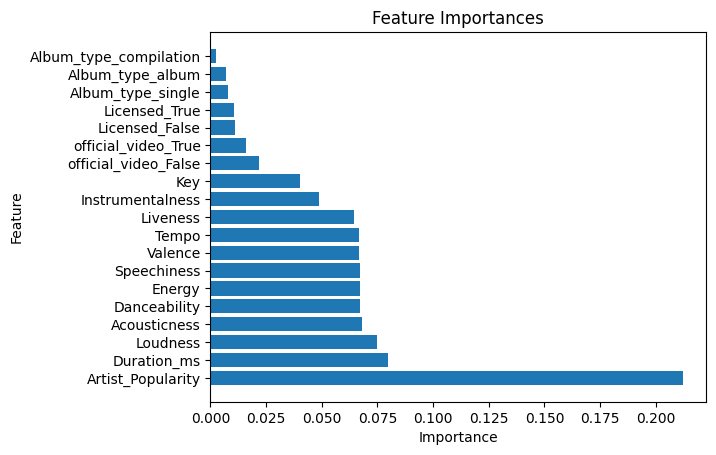
\includegraphics[width=.8\linewidth]{feature_importance.png}
	\caption{Feature importance for Random Forest}\label{fig:feature_importance}
\end{figure}

By examining the feature importances, it was observed that the "Artist Popularity" feature exhibited relatively higher importance compared to the other features used in the model. This indicates that the "Artist Popularity" feature contributes significantly to the classification of song popularity and provides valuable information for the model to make accurate predictions.

\newblock

Still in the endeavor to enhance the classification results, threshold-based feature selection was performed, where a range of threshold values was defined to select features based on their importance. By iteratively adjusting the threshold, the most influential features were identified and included in the model.

To implement the feature selection process, a mask was created to select only the features with importance greater than or equal to the threshold value. This allowed for a more focused model that leveraged the most relevant features in predicting song popularity. By considering only the important features, the model was able to reduce noise and potentially improve its ability to capture the underlying patterns and relationships within the data.

Hyperparameter tuning was another crucial step in enhancing the model's performance. A parameter grid was defined to explore different combinations of hyperparameters, such as "n\_estimators" and "max\_depth", which were specific to the Random Forest algorithm.

GridSearchCV, a technique for hyperparameter optimization, was employed to perform a systematic search across the parameter grid using only the selected features. This process aimed to find the best combination of hyperparameters that maximized the model's performance.

Once the best parameters were determined through the grid search, a new Random Forest model, rf\_classifier, was created using these optimized parameters. This ensured that the model was configured with the most suitable settings for the given dataset and task.

The model was then retrained using only the selected features, allowing it to focus on the most informative aspects of the data. The retrained model was subsequently used to predict the target variable on the test set, generating the predicted values, y\_pred. By using the selected features and the optimized parameters, the model aimed to provide more accurate predictions of song popularity.

\begin{table}[H]
	\centering
	\begin{tabular}{lcccc}
		\toprule
		\textbf{Popularity Level} & \textbf{Precision} & \textbf{Recall} & \textbf{F1-Score} & \textbf{Support} \\
		\midrule
		\hline
		0                         & 0.51               & 0.38            & 0.43              & 806              \\
		1                         & 0.63               & 0.65            & 0.64              & 1116             \\
		2                         & 0.57               & 0.65            & 0.61              & 1612             \\
		3                         & 0.66               & 0.58            & 0.62              & 376              \\
		\hline
		Accuracy                  & -                  & -               & 0.59              & 3910             \\
		Macro Avg                 & 0.59               & 0.57            & 0.58              & 3910             \\
		Weighted Avg              & 0.58               & 0.59            & 0.58              & 3910             \\
		\bottomrule
	\end{tabular}
\end{table}

Now the Random Forest model performed better compared to the previous Random Forest model. It achieved an overall accuracy of 0.59, correctly predicting 59a\% of the instances in the test set. The precision, recall, and F1-scores for each popularity level were generally higher compared to the previous Random Forest results.

Although these values are better than the previous, and definitely better than random guessing, they do not provide confidence about the classification result. 

\newblock

Discussion:

The classification of popularity based solely on sound features can be a challenging task, as evidenced by the performance of the implemented models. Several reasons contribute to this challenge.

Firstly, popularity is inherently subjective, varying among individuals. It is influenced by personal preferences, cultural context, and social trends. Sound features alone may not fully capture these subjective aspects that contribute to the perception of popularity. Different listeners may have diverse interpretations of what makes a song popular, leading to inconsistencies in the classification results.

Secondly, the concept of popularity is complex and multifaceted. It is influenced by various factors, including melody, lyrics, rhythm, production quality, and artist popularity. These factors interact in intricate ways, making it challenging to capture their relationships solely based on sound features. The models implemented in this study might not have adequately captured the intricate patterns and interplay of these factors, resulting in suboptimal classification performance.

Moreover, contextual factors play a crucial role in determining the popularity of a song. Marketing strategies, media exposure, and cultural events can significantly impact a song's popularity, even surpassing the influence of sound features. Unfortunately, sound features alone might not encompass these contextual factors, limiting the models' ability to accurately classify popularity.

In conclusion, while machine learning models based on sound features provide valuable insights, they face inherent limitations when it comes to classifying popularity. The subjective nature of popularity, the complexity of its influencing factors, and the influence of contextual factors all contribute to the challenges faced in accurately predicting popularity based solely on sound features. Future research could explore incorporating additional data sources, such as social media trends, user preferences, or external contextual information, to improve the classification performance and provide a more comprehensive understanding of popularity.

\newpage

\begin{thebibliography}{9}
	\bibitem{Rasetri} Rastelli, S. (2020). Spotify and YouTube. Retrieved from \href{https://www.kaggle.com/datasets/salvatorerastelli/spotify-and-youtube}{https://www.kaggle.com/datasets/salvatorerastelli/spotify-and-youtube} (Accessed: July 5, 2023).\\
	\bibitem{spotifyApi} Spotify Developer API. Retrieved from \href{https://developer.spotify.com/documentation/web-api/reference/get-audio-features}{https://developer.spotify.com/documentation/web-api/reference/get-audio-features} (Accessed: July 5, 2023).\\
	\bibitem{CambridgeDictionary} Cambridge Dictionary. Retrieved from \href{https://dictionary.cambridge.org/dictionary/english/popularity}{https://dictionary.cambridge.org/dictionary/english/popularity} (Accessed: July 5, 2023).\\
	\bibitem{CollinsDisctionary} Collins Dictionary. Retrieved from \href{https://www.collinsdictionary.com/dictionary/english/popularity}{https://www.collinsdictionary.com/dictionary/english/popularity} (Accessed: July 5, 2023).\\
	\bibitem{WikipediaPopularity} Wikipedia. Retrieved from \href{https://en.wikipedia.org/wiki/Popularity}{https://en.wikipedia.org/wiki/Popularity} (Accessed: July 5, 2023).\\
	\bibitem{LongTail} Wikipedia. Retrieved from \href{https://en.wikipedia.org/wiki/Long_tail}{https://en.wikipedia.org/wiki/Long\_tail} (Accessed: July 5, 2023).\\
\end{thebibliography}

\end{document}
